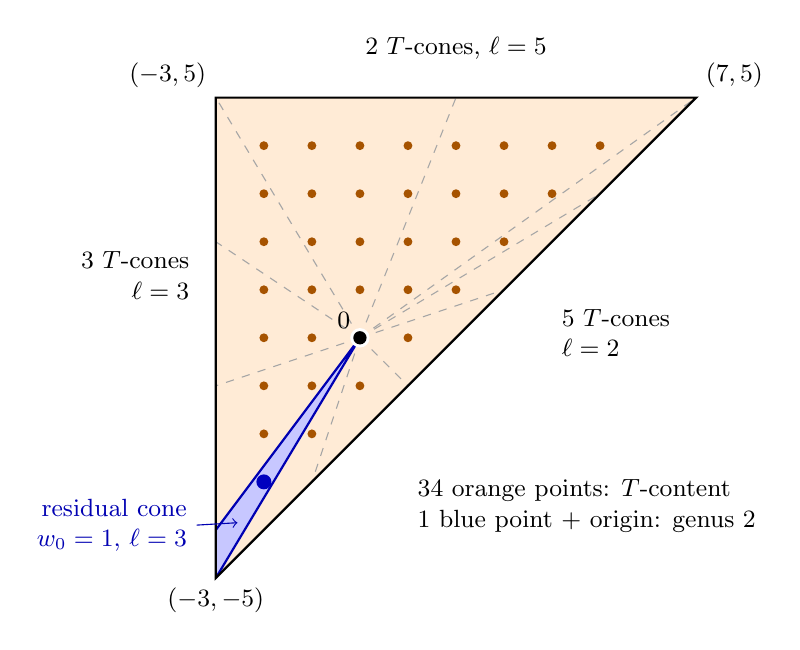
\begin{tikzpicture}[x=0.61cm,y=0.61cm,font=\small]
  \fill[orange!16] (-3,-5)--(7,5)--(-3,5)--cycle;
  \fill[blue!22] (0,0)--(-3,-4)--(-3,-5)--cycle;
  \foreach \horizontal/\vertical in {-3/-5,-1/-3,1/-1,3/1,5/3,7/5,2/5,-3/5,-3/2,-3/-1,-3/-4}
    \draw[gray!70,dashed,thin] (0,0)--(\horizontal,\vertical);
  \draw[blue!70!black,thick] (-3,-4)--(0,0)--(-3,-5);
  \draw[thick] (-3,-5)--(7,5)--(-3,5)--cycle;
  \foreach \horizontal/\lowest in {-2/-3,-1/-2,0/-1,1/0,2/1,3/2,4/3,5/4}
    \foreach \vertical in {\lowest,...,4}
      \fill[orange!65!black] (\horizontal,\vertical) circle (1.6pt);
  \fill[blue!75!black] (-2,-3) circle (2.7pt);
  \fill[white] (0,0) circle (3.5pt);
  \fill (0,0) circle (2.4pt) node[above left] {$0$};
  \node[above left] at (-3,5) {$(-3,5)$};
  \node[above right] at (7,5) {$(7,5)$};
  \node[below] at (-3,-5) {$(-3,-5)$};
  \node[above,align=center] at (2,5.6) {$2$ $T$-cones, $\ell=5$};
  \node[anchor=east,align=right] at (-3.35,1.3) {$3$ $T$-cones\\$\ell=3$};
  \node[anchor=west,align=left] at (4,0.1) {$5$ $T$-cones\\$\ell=2$};
  \node[anchor=east,align=right,text=blue!70!black] at (-3.4,-3.9) {residual cone\\$w_0=1$, $\ell=3$};
  \draw[blue!70!black,->] (-3.4,-3.9)--(-2.55,-3.85);
  \node[anchor=west,align=left] at (1,-3.5)
    {$34$ orange points: $T$-content\\
     $1$ blue point $+$ origin: genus $2$};
\end{tikzpicture}